\documentclass[11pt]{standalone}

\usepackage{lmodern}	% font definition
\usepackage{amsmath}	% math fonts
\usepackage{amsthm}
\usepackage{amsfonts}
\usepackage{pgfplots}

\usepackage{pgfplots}
\usepackage{xcolor}
\usetikzlibrary{positioning,bayesnet}
\definecolor{brinkpink}{rgb}{0.98, 0.38, 0.5}
\definecolor{aogreen}{rgb}{0.0, 0.5, 0.0}
\usepackage{tikz}
\usetikzlibrary{decorations.pathmorphing} % noisy shapes
\usetikzlibrary{fit}					% fitting shapes to coordinates
\usetikzlibrary{backgrounds}	% drawing the background after the foreground
\pgfplotsset{compat=newest}% <-- moves axis labels near ticklabels (respects tick label widths)

\begin{document}
  \pgfplotsset{every tick label/.append style={font=\normalsize}}
  \pgfplotsset{every axis label/.append style={font=\normalsize}}
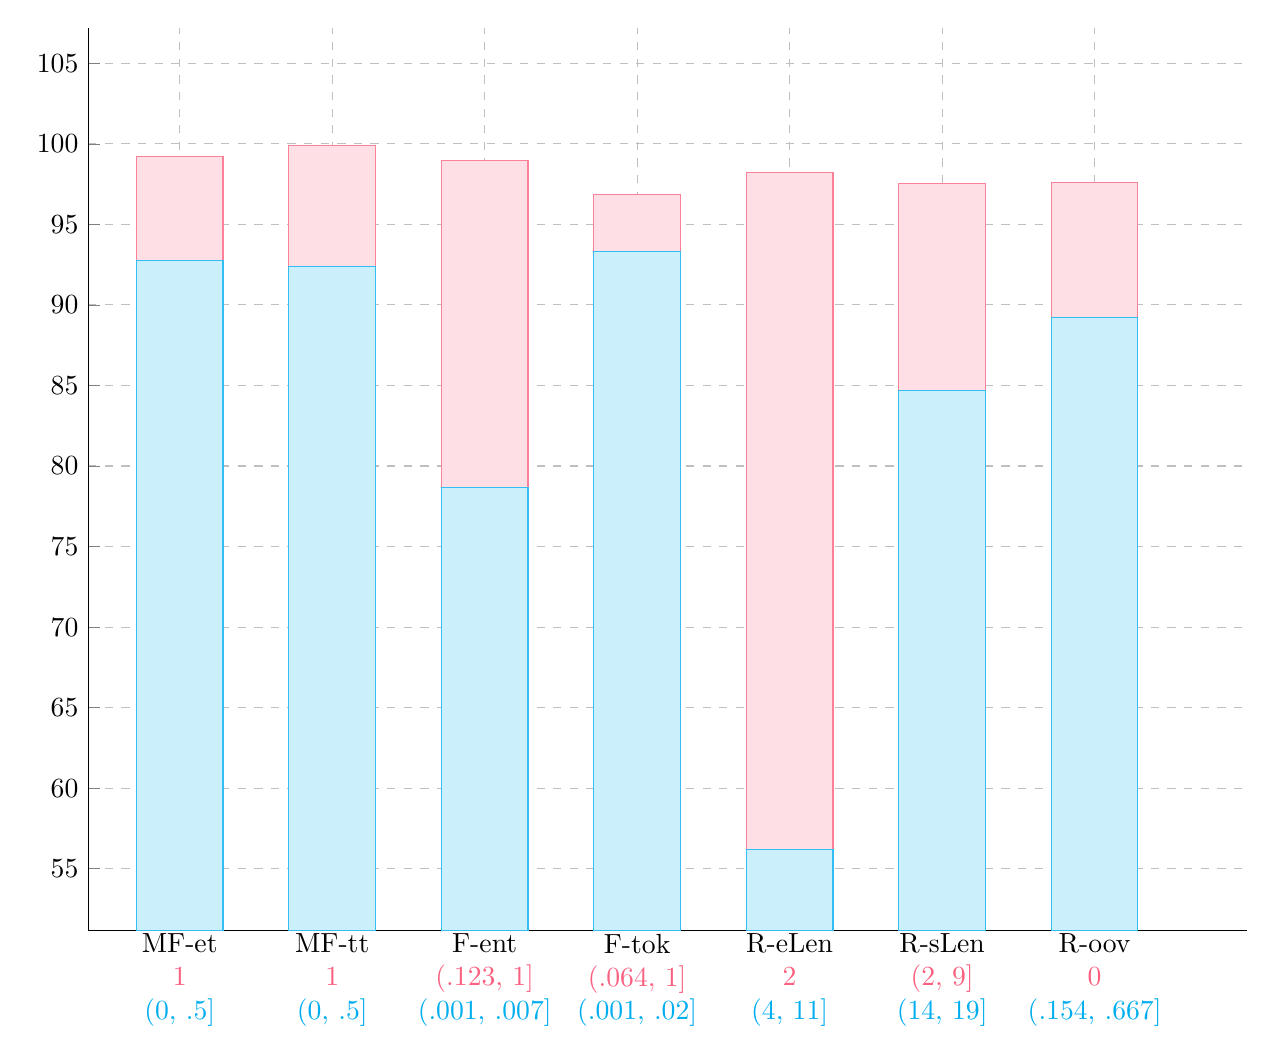
\begin{tikzpicture}
  \centering
  \begin{axis}[%ybar=1.0pt,
    ybar stacked,
    height=13.040000000000001cm,
    %width=16.3cm, % 12->9,  9->6.93,  8-> 6
    width=16.3cm, % 12->9,  9->6.93,  8-> 6
    bar width=1.1cm,
    xmin=0.4,
    xmax=8,
    ymin=51.17,
    ymax=99.87,
    enlarge y limits={upper,value=0.15},
    axis lines*=left,
    legend style={at={(0.5,-0.25)},anchor=north,legend columns=-1,
    /tikz/every even column/.append style={column sep=0.2cm}},
    %xticklabels={\textcolor{brinkpink}{S}-\textcolor{aogreen}{L},\textcolor{brinkpink}{M}-\textcolor{aogreen}{S},\textcolor{brinkpink}{L}-\textcolor{aogreen}{M},\textcolor{brinkpink}{S}-\textcolor{aogreen}{S},\textcolor{brinkpink}{M}-\textcolor{aogreen}{M},\textcolor{brinkpink}{L}-\textcolor{aogreen}{L},\textcolor{brinkpink}{S}-\textcolor{aogreen}{S},\textcolor{brinkpink}{M}-\textcolor{aogreen}{M}},
    xticklabels={MF-et \\ \textcolor{brinkpink}{1} \\ \textcolor{cyan}{(0, .5]}, MF-tt \\ \textcolor{brinkpink}{1} \\ \textcolor{cyan}{(0, .5]}, F-ent \\ \textcolor{brinkpink}{(.123, 1]} \\ \textcolor{cyan}{(.001, .007]}, F-tok \\ \textcolor{brinkpink}{(.064, 1]} \\ \textcolor{cyan}{(.001, .02]}, R-eLen \\ \textcolor{brinkpink}{2} \\ \textcolor{cyan}{(4, 11]}, R-sLen \\ \textcolor{brinkpink}{(2, 9]} \\ \textcolor{cyan}{(14, 19]}, R-oov \\ \textcolor{brinkpink}{0} \\ \textcolor{cyan}{(.154, .667]}},
    xtick=data,
    xmajorgrids=true,
    ymajorgrids=true,
    zmajorgrids=true,
    grid style=dashed,
    xticklabel style={
        inner sep=1pt,
	align=center,
        %rotate=90,
        %anchor=near xticklabel,
    },
    ]
    %\addplot [draw=aogreen!80,fill=aogreen!20] table[x=id,y=y]{
    \addplot [draw=cyan!80,fill=cyan!20] table[x=id,y=y]{
    id  y
    	1	92.77
	2	92.36
	3	78.65
	4	93.3
	5	56.17
	6	84.69
	7	89.23
    };
    \addplot [draw=brinkpink!80,fill=brinkpink!20] table[x=id,y=y]{
    id  y
    	1	6.42
	2	7.52
	3	20.32
	4	3.57
	5	42.06
	6	12.83
	7	8.39
    };
  \end{axis}
\end{tikzpicture}

\end{document}

